\documentclass{article}
\usepackage{graphicx} % Required for inserting images
\usepackage{amsmath, bm, mathtools, amsfonts, amssymb}
\usepackage{xcolor}
\usepackage{adjustbox} 
\usepackage{hhline}

\newcommand{\diff}{\mathop{}\!\mathrm{d}}

\usepackage{tikz}
\usetikzlibrary{decorations.pathreplacing,calligraphy}
\usetikzlibrary{positioning}
\usetikzlibrary{positioning,shapes.symbols,fit}
\tikzset{
	roundnode2/.style={circle, draw=green!50!blue, very thick, minimum size=9mm}
}
%\usetikzlibrary{shapes, arrows, calc, arrows.meta, fit, positioning}
%\usetikzlibrary{arrows.meta}
\tikzset{
	roundnode/.style={circle, draw=green!50!blue, fill=green!60!blue, very thick, minimum size=7mm},
	rectnode/.style={rectangle, draw=green!50!blue, very thick, minimum size=8.5mm},
	mydotted/.style = {dash pattern=on 6.1pt off 7pt}
}


%\usepackage[backend=bibtex,style=numeric,natbib=true,maxbibnames=5,giveninits=true]{biblatex}
\usepackage[backend=bibtex,style=numeric,natbib=true,maxbibnames=5,giveninits=true]{biblatex}
\newcommand*{\bibtitle}{References}
\DeclareNameAlias{default}{last-first}
\addbibresource{bib.bib}

\title{Efficient inference in a weakly non-linear Bayesian inverse Problem using an affine approximation}
\author{Lennart Golks and Colin Fox}
\date{November 2025}

\begin{document}

\maketitle

\section{Introduction}
There are satellites, which orbit around the earth at a height of around 500km above the ground, carry measurement devices to determine trace gas concentrations in the stratosphere.
More specifically, atmospheric limb-sounders are pointing through the atmosphere and detect thermal radiation of trace gases, e.g., ozone.
Examples of such limb-sounders are the Microwave
Limb Sounder (MLS) on NASA’s Aura mission~\cite{waters2006earth} and the
Michelson Interferometer for Passive Atmospheric Sounding
(MIPAS) on ESA’s Envisat~\cite{readings2000envisat}.

Measurements of such devices can be described by the radiative transfer equation (RTE), which in this case is a path integral along the satellite's pointing direction.
This path integral includes an absorption term accounting for the re-attenuation of the thermal radiation along the satellite's line of sight.
That makes inferring the trace gas concentration from a set of measurements a non-linear inverse problem.

Existing methods use regularisation methods to retrieve trace gas concentration from measurements~\cite{rodgers1976retrieval, livesey2006retrieval, raspollini2021level}.
These methods do not include hyper-parameters, such as noise covariance, and produce biased results~\cite{Froidevaux2008snrozone}.

Firstly, given some simulated data, we treat this non-linear problem as a linear problem by neglecting the absorption term in the RTE.
A linear-Gaussian hierarchical Bayesian framework is employed to infer the ozone concentration in the stratosphere.
This includes establishing a hierarchical structure and classifying hyper-parameters and parameters.
For efficient inference we employ the marginal-and-then-conditional (MTC) scheme as in~\cite{fox2016fast}.
This gives a low-dimensional marginal posterior probability distribution over the hyper-parameters and a high-dimensional conditional posterior probability for the ozone parameter.
We show that evaluating the marginal posterior on a grid gives the conditional posterior mean at no additional cost.
To quantify the conditional posterior variance, samples from the conditional posterior are drawn via the randomise-then-optimise (RTO) scheme~\cite{bardsley2012mcmc}.

Using the results of the linearised problem, an affine map approximating the non-linear forward model is obtained.
We employ the same hierarchical Bayesian framework as previously used, but with the approximated forward model, to quantify the unbiased mean and variance of the posterior ozone profile.

All programming and analysis in this paper are done in Python, and the reported computation times are taken on a MacBook Pro from 2019 with a 2.4 GHz quad-core Intel i5 processor.

\section{Hierarchical Bayesian Modelling}
\label{sec:BayesIntro}
First, the concept of hierarchical Bayesian modelling is introduced.
Assume we observe some data
\begin{align}
	\bm{y} = \bm{A}( \bm{x}) + \bm{\eta},
	\label{eq:NonLinDat}
\end{align}
based on the forward model $\bm{A}(\bm{x})$ with an unknown parameter vector $\bm{x}$ and some additive random noise $\bm{\eta}$.
Naturally, due to the noise, the observation process in Eq. \ref{eq:NonLinDat} is a random process.
Hence, in Bayesian modelling, the aim is to determine a probability distribution over the parameter $\bm{x}$ given some data $\bm{y}$.
Further, a hierarchical Bayesian model incorporates (auxiliary) hyper-parameters $\bm{\theta}$ (see Fig.~\ref{fig:FirstDAG} for a schematic represntation).
Within a Bayesian approach all unknown hyper-parameters and parameters are treated as random variables~\cite[Chapter 3]{kaipio2005statinv}.
\begin{figure}[ht!]
	\centering
	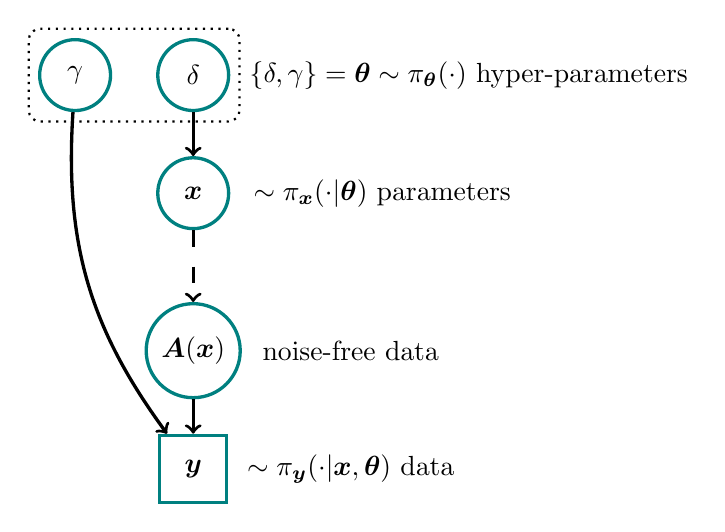
\begin{tikzpicture}
		
		every edge/.style = {draw, -latex, thick} % <---
		\node[roundnode2] at (0,2) (del)    {$\delta$};
		\node[roundnode2] at (-1.5,2) (gam)    {$\gamma$};
		%\node[align=center] at (-0.75,2.25) (theta) {$\bm{\theta}$};
		\node[roundnode2] at (0,0.5) (x)    {$\bm{x}$};
		\node[roundnode2] at (0,-1.5) (u)    {$\bm{A}(\bm{x})$};
		\node[rectnode] at (0,-3) (y)    {$\bm{y}$};
		
		%\node[align=center] at (-3.25,0) (nt) {noise\\$\bm{\eta} \sim$};
		
		\draw[->, very thick, mydotted] (x.south) -- (u.north); 
		\draw[->, very thick] (u.south) -- (y.north); 
		\draw[->, very thick] (del.south) -- (x.north); 
		\draw[->, very thick] (gam) edge[bend right=20] (y);  
		
		\node[align=center] at (3.5,2) (tht) {$\{\delta, \gamma\} = \bm{\theta}\sim \pi_{\bm{\theta}}(\cdot) $ hyper-parameters};
		\node[align=center] at (2.4,0.5) (xt) {$\sim \pi_{\bm{x}}(\cdot|\bm{\theta}) $ parameters};
		\node[align=center] at (2,-1.5) (ut) {noise-free data};
		\node[align=center] at (2,-3) (yt) {$\sim \pi_{\bm{y}}(\cdot|\bm{x},\bm{\theta})$ data};
		%\node[align=center] at (-3.25,0) (nt) {noise\\$\bm{\eta} \sim \pi_{\bm{\eta}}(\cdot|\bm{\theta})$};
		%\node[fit=(s)(d),draw,dotted,black, rounded corners] {};
		\node[fit=(del)(gam),draw,thick,dotted,black, rounded corners] {};
	\end{tikzpicture}
	\caption[Hierarchical Bayesian Model]{\textcolor{red}{A directed acyclic graph (DAG) for an inverse problem visualises statistical dependencies as solid line arrows and deterministic dependencies as dotted arrows.
		The hyper-parameters $\bm{\theta}$ are distributed as ($\sim$) the hyper-prior distribution $\pi(\bm{\theta})$.
		The prior distribution $ \pi_{\bm{x}}(\cdot|\bm{\theta})$ for the parameter $\bm{x}$ and the noise  $\bm{\eta} \sim \pi_{\bm{\eta}}(\cdot|\bm{\theta})$ are statistically dependent on some of those hyper-parameters.
		Then a parameter $\bm{x} \sim \pi_{\bm{x}}(\cdot|\bm{\theta})$ is deterministically mapped through the forward model $\bm{A}(\bm{x})$.
		Based on the noise-free data we observe (square box) a data set $\bm{y} = \bm{A}(\bm{x}) + \bm{\eta}$ with some additive random noise, which determines the likelihood function $\pi(\bm{y}|\bm{x},\bm{\theta})$.}}
	\label{fig:FirstDAG}
\end{figure}

According to Bayes' theorem, the joint posterior distribution over the parameters $\bm{x}$ and the hyper-parameter $\bm{\theta}$ is given as
\begin{align}
	\pi(\bm{x},\bm{\theta}|\bm{y}) = \frac{ \pi(\bm{y} | \bm{x}, \bm{\theta} ) \pi(\bm{x}, \bm{\theta})}{\pi(\bm{y})} \propto \pi(\bm{y} | \bm{x}, \bm{\theta} ) \pi(\bm{x}, \bm{\theta}) \, ,
\end{align}
with finite and non-zero $\pi(\bm{y})$.
The likelihood function $\pi(\bm{y}|\bm{x},\bm{\theta})$ is defined by the nature of the noise and the noise-free data $\bm{A}(\bm{x})$, which we read as the distribution over $\bm{y}$ conditioned on $\bm{x}$ and $\bm{\theta}$.
Here $\bm{\theta}$ describe multiple hyper-parameters, e.g.~the noise precision so that $\bm{\eta} \sim \pi_{\bm{\eta}}(\cdot|\bm{\theta})$, where $\sim$ reads as ``is distributed as''.
Further, $\bm{\theta}$ may account for some physical properties of $\bm{x}$ such as the smoothness (see Sec.~\ref{sec:BayModel}).
Because all unknown parameter are treated as random variables the joint prior distribution is introduced as $\pi(\bm{x}, \bm{\theta}) = \pi(\bm{x}|\bm{\theta}) \pi(\bm{\theta})$ with the parameter prior distribution $\pi(\bm{x}|\bm{\theta})$ and the hyper-prior distribution $\pi(\bm{\theta})$.
Choosing these prior distributions is ultimately a modeller's choice and is crucial, as those shall be as uninformative as possible for regions in hyper-parameter and parameter space where the data is informative.
If the data is uninformative, the prior distributions can be informative and may represent a rather restrictive range of (physically) feasible hyper-parameters and parameters.

We can write the hierarchical model as:
\begin{subequations}
	\begin{align}
		\bm{y} |  \bm{x},\bm{\theta}  &\sim \pi(\bm{y} | \bm{x}, \bm{\theta} ) \\
		\bm{x}| \bm{\theta}   &\sim \pi(\bm{x}|\bm{\theta})   \\
		\bm{\theta}   &\sim \pi(\bm{\theta} ) \, .
	\end{align} 
\end{subequations}
Usually, the objective is to calculate the expectation of a function $h(\bm{x})$, which is defined as
\begin{align}
	\text{E}_{\bm{x},\bm{\theta}|\bm{y}} [h(\bm{x})] =  \int \int   h(\bm{x}) \,  \pi(\bm{x}, \bm{\theta} | \bm{y} ) \, \diff \bm{x}  \, \diff \bm{\theta}  \label{eq:expPos} \, .
\end{align}
\subsection{Marginal-then-Conditional Method}
\label{subsec:TheoMTC}
Characterising the posterior distribution or quickly generating a representative sample set from the posterior distribution often presents a significant challenge. 
This is mainly due to the strong correlations that usually exist between the parameters $\bm{x}$ and hyper-parameters $\bm{\theta}$, as discussed by Rue and Held in~\cite{rue2005gaussian}.

Depending on the problem and the available model, it is beneficial to factorise the joint posterior distribution
\begin{align}
	\pi(\bm{x}, \bm{\theta} |  \bm{y}) = \pi(\bm{x} |  \bm{\theta}, \bm{y}) \, \pi(\bm{\theta} |   \bm{y}) \label{eq:MTC}
\end{align}
into the full conditional posterior $\pi(\bm{x} |  \bm{\theta}, \bm{y})$ over the latent field $\bm{x}$ and the marginal posterior $ \pi(\bm{\theta} |   \bm{y})$ over hyper-parameter $\bm{\theta}$.
This approach, known as the marginal-and-then-conditional (MTC) method~\cite{fox2016fast}, is particularly advantageous when $\bm{x}\in \mathbb{R}^n$ is high-dimensional, while $\bm{\theta}$ is low-dimensional and the evaluation of the marginal posterior
\begin{align}
	\pi(\bm{\theta} |   \bm{y}) =  \frac{ \pi(   \bm{y} | \bm{x},\bm{\theta})  \pi( \bm{x} | \bm{\theta} )  \pi(\bm{\theta}) }{ \pi(\bm{x} | \bm{\theta} ,   \bm{y})   \pi( \bm{y})} \propto \frac{ \pi(   \bm{y} | \bm{x},\bm{\theta})  \pi( \bm{x} | \bm{\theta} )  \pi(\bm{\theta}) }{ \pi(\bm{x} | \bm{\theta} ,   \bm{y}) } \label{eq:margGen}\, 
\end{align}
as in~\cite[Lemma 2]{fox2016fast} is relatively cheap.
Applying the law of total expectation~\cite{champ2022generalizedlawtotalcovariance}, Eq.~\eqref{eq:expPos} becomes
\begin{align}
	\mathbb{E}_{\bm{x} ,\bm{\theta}  |\bm{y}} [h(\bm{x})] &= \int \int   h(\bm{x}) \pi(\bm{x} |  \bm{\theta}, \bm{y}) \, \diff \bm{x} \,  \pi(\bm{\theta} |   \bm{y}) \, \diff \bm{\theta} \\
	&= \int \mathbb{E}_{\bm{x} |  \bm{\theta}, \bm{y}} \left[ h(\bm{x}) \right] \, \pi(\bm{\theta} |  \bm{y}) \, \diff \bm{\theta}\label{eq:2fullCond} \\
	&= \mathbb{E}_{\bm{\theta} |  \bm{y}} \left[ \mathbb{E}_{\bm{x} |  \bm{\theta}, \bm{y}} [h(\bm{x})] \right] \, .
	\label{eq:fullCond}
\end{align}

In the case of a linear-Gaussian hierarchical Bayesian model, both the marginal distribution $\pi (\bm{\theta}| \bm{y})$ 
and the inner expectation $\mathbb{E}_{\bm{x} |  \bm{\theta}, \bm{y}} \left[ h(\bm{x}) \right]$ are well defined (see Sec.~\ref{sec:BayModel} and \cite{fox2016fast}).
If the integral in Eq.~\ref{eq:2fullCond} is expensive to calculate sample-based methods may be used to calculate the expectations in 
Eq.~\eqref{eq:2fullCond}.
To produce samples $\{ (\bm{x}, \bm{\theta})^{(1)}, \dots, (\bm{x}, \bm{\theta})^{(k)}, \dots, (\bm{x}, \bm{\theta})^{(N)} \} \sim \pi(\bm{x}, \bm{\theta} |  \bm{y}) $ one needs an independent sample from $\bm{\theta}^{(k)} \sim \pi(\bm{\theta} |  \bm{y})$ first and then draws a sample from the full conditional posterior $\bm{x}^{(k)} \sim \pi(\bm{x} | \bm{\theta}^{(k)}  , \bm{y})$.

\textcolor{red}{
Note that for the affine case, where e.g., the forward model is given by $\bm{A}\bm{x} + \bm{b}$, the MTC method as in \cite{fox2016fast} is still applicable.
For Gaussian noise and a Gaussian prior, the form of the posterior of the affine case does not change compared to the linear-Gaussian case, where the forward model may be given by $\bm{A}\bm{x}$.}
\section{The Forward Model}
\label{ch:formodel}
Here we present the forward model to which we apply the methodology.
The forward model describes a Limb-sounder measuring thermal radiation of ozone to determine the atmospheric ozone concentration.
We follow the MIPAS handbook~\cite{mipas2000handbook} and simulate data according to an idealised cloud-free atmosphere in local thermodynamic equilibrium, assuming a measurement instrument with infinite spectral resolution and no pointing errors.
This is a simplified forward model.
No other instrument-specific details such as sensor area or antenna response are included because they are not available to us. 

\begin{figure}[ht!]
	\centering
	\input{LIMB.pdf_tex}
	\caption[Schematic of measurement and analysis geometry.]{Schematic of measurement and analysis geometry, not to scale.
		The stationary satellite, at a constant height $h_\text{sat}$ above Earth, takes $m$ measurements along its line-of-sight defined by the line $\Gamma_j$.
		Each measurement has a pointing angle $\phi_j$ and a tangent height $h_{\ell_j}$, $j=1,2,\dots,m$ defined as the closest distance of $\Gamma_j$ to the Earth's surface.
		Between $h_{L,0} \approx 7$km and $h_{L,n} \approx 83$km, the atmosphere is discretised into $n$ layers as illustrated by the solid green lines.}
	\label{fig:LIMB}
\end{figure}
As displayed in Fig.~\ref{fig:LIMB}, a satellite at a constant height $h_{\text{sat}}$ is pointing through the atmosphere (limb-sounding) to measure thermal radiation of ozone.
For each measurement $j=1,2,\ldots,m$, the tangent height $h_{\ell_j}$ and the corresponding line-of-sight $\Gamma_j$ are defined.
Additionally, we introduce the pointing angle $0 \leq \phi_j < \phi_{\text{max}}$, so that if $\phi = 0 \text{arc sec}$ the satellite points at $h_{L,0}$ and for a pointing angle $\phi_{\text{max}}$ at $h_{L,n}$.
Further, the atmosphere is discretised into $n$ layers defined by height values $h_{L,i-1} < h_{L,i}$ with respect to the surface of the Earth, for $i = 1, \dots, n$.
More specifically, the $i$-th layer is defined by two spheres around the centre of the Earth with radii $ r_0 + h_{L,i-1} $ and $r_0 + h_{L,i}$, where $r_0$ is the Earth's radius.
Within a layer the signal is constant, whereas above $h_{L, n}$ and below $h_{L,0} $ no signal can be obtained.


\subsection{Radiative Transfer Equation}
\label{sec:RTE}
One noise-free measurement of thermal radiation emitted by gas molecules within the atmosphere is described by the radiative transfer equation (RTE)~\cite{mipas2000handbook}
\begin{align}
	\label{eq:RTE} 
	  \int_{\Gamma_j}  B(\nu,T) k(\nu, T)   \frac{p(r)}{k_{\text{B}} T(r)}  x(r)  \tau(r) \text{d}r \,  \\
\text{with } \,	\tau(r) = \exp{ \Bigl\{ - \int^{r}_{r_\text{obs}}  k(\nu, T)   \frac{p(r^{\prime})}{k_B T(r^{\prime})}  x(r^{\prime}) \text{d}r^{\prime} \Bigr\} } \, \label{eq:absRTE} .
\end{align}
This is a path integral along the satellite's straight line of sight $\Gamma_j$ with the ozone volume mixing ratio (VMR) $x(r)$ at distance $r$ from the satellite, at the wave number $\nu$.
Within the atmosphere, the number density $p(r) / (k_{\text{B}} T(r))$ of molecules is dependent on the pressure $p(r)$, the temperature $T(r)$, and the Boltzmann constant $k_{\text{B}}$.
The factor $\tau(r)\leq 1$ accounts for re-absorption of the radiation along the line-of-sight, which makes the RTE non-linear.
The absorption constant is given as
\begin{align}
	k(\nu, T) = L(\nu, T_{\text{ref}}) \frac{Q(T_{\text{ref}})}{Q(T)} \frac{ \exp{\{ - c_2 E^{\prime \prime} / T\}} }{\exp{\{ - c_2 E^{\prime \prime} / T_{\text{ref}} \}}} \frac{ 1- \exp{\{ - c_2 \nu  / T \}} }{1 - \exp{\{ - c_2 \nu / T_{\text{ref}} \}}}
\end{align}
with Planck's constant $h$ and speed of light $c$.
The line intensity $L(\nu, T_{\text{ref}})$ at reference temperature $T_{\text{ref}} =296K $, the lower-state energy $ E^{\prime \prime} $ in $\text{cm}^{-1}$ of the targeted transition and the second radiation constant $c_2\coloneqq hc/k_{\text{B}} \approx 1.44\text{cmK}$ are provided by the HITRAN database~\cite{gordon2022hitran2020}.
The total internal partition function is given as
\begin{align}
	Q(T )= g^{ \prime} \exp{\{ - \frac{ c_2 E^{ \prime} }{T}\}} + g^{\prime \prime} \exp{\{ - \frac{ c_2 E^{\prime \prime} }{T}\}} \, ,
\end{align}
with the statistical weight $ g^{\prime \prime}$ for the lower and $ g^{ \prime}$ for the upper energy state (also called the degeneracy factors) accounting for the molecule's non-rotational and rotational energy states (see also~\cite{vsimevckova2006einstein}), and the upper state energy $E^{ \prime} = E^{ \prime\prime} + \nu$.
Under the assumption of local thermodynamic equilibrium (LTE), the black body radiation acts as a source function
\begin{align}
	B(\nu,T)   = \frac{2 h c^2 \nu^3}{\exp{\{\frac{c_2\nu}{ T}\}}-1}\, .
\end{align}
For fundamentals on the RTE, we recommend~\cite[Chapter 1]{rybicki2000rte}, and for a more comprehensive model, we refer to \cite{read2006forwardModel}.

When simulating data, we assume an idealised limb-sounder.
Since the measurement device has a negligible frequency window, the line broadening around $\nu$ for the calculations of $L(\nu, T_{\text{ref}})$ is neglected.
Normally, this is modelled as the convolution of the normalised Lorentz profile (collisional/pressure broadening) and the normalised Doppler profile (thermal broadening)~\cite{mipas2000handbook}.
Additionally, we target one specific molecule and calculate $k(\nu, T)$ accordingly.
Usually, this would involve a summation over the individual absorption constants for multiple radiating molecules weighted by their respective VMR~\cite{mipas2000handbook}.


\subsection{Simulated Data and Ground Truth}
\label{sec:SimDat}
As the ground truth for our methodology, we consider an ozone profile at distinct pressure values generated from some data~\cite{MLSdata} of the MLS on the Aura satellite within the Antarctic region.
This ozone profile has a peak in the middle atmosphere and a second peak at higher altitudes, see Fig.~\ref{fig:OzonSampl}, which seems to be a typical nighttime profile~\cite{Lee2020NightOzone}.
For more information on the processes within the atmosphere for ozone, we refer to~\cite{Lee2020NightOzone}.

We can relate the height $h$ and the pressure values $p$ via the hydrostatic equilibrium equation
\begin{align}
	\text{d}(\log p) = \frac{\text{d}p}{p} = \frac{- g M}{R^* T} \text{d} h \, .\label{eq:hydr}
\end{align}
Here the acceleration due to gravity is $g$, the universal gas constant is $R^* = 8.31432 \times 10^{-3} \text{Nm} / \text{kmol} / \text{K}$ and the mean molecular weight of the air is $M = 28.97 \text{kg/kmol}$, as in~\cite{atmosphere1976us}.
To enable efficient calculation of the RTE we discretise the atmosphere as in Fig.~\ref{fig:LIMB}.
Then the ozone VMR $\bm{x} =\{x_1,x_2,\ldots,x_n\} \in \mathbb{R}^{n}$, pressure $\bm{p} =\{p_1,p_2,\ldots,p_n\} \in \mathbb{R}^{n}$ and temperature $\bm{T} =\{T_1,T_2,\ldots,T_n\} \in \mathbb{R}^{n}$, as well as all other height dependent parameters, are discretised profiles with constant values between the heights $h_{L,i-1} \leq h < h_{L,i}$, for each layer $i = 1,\dots, n$.
The hydrostatic equilibrium equation for the discretised atmosphere is
\begin{align}
	h_{L,i} =  h_{L,i-1} - \frac{\Delta p R^* T_{i-1}  }{p_{i-1}  g_{i-1} M} \, 
\end{align}
with $\Delta p = p_{i} - p_{i-1}$ and $T_{i-1} = T(h_{i-1})$ as in Eq.~\ref{eq:tempFunc} (see also~\cite{Carlotti99,Ridolfi00}), for $i = 1,\dots, n$.
At sea level $h = 0$km the mean pressure is $p_0 = 1013.25$hPa and the mean temperature is $T_0 = 288.15$K~\cite{atmosphere1976us}.
The acceleration due to gravity is
\begin{align}
	g_i = g_0 \Bigg( \frac{r_0}{r_0 + h_{L,i}} \Bigg) \, ,
\end{align}
where the polar radius of the Earth is $r_0 \approx 6356 \, \text{km}$, the gravitation at sea level is $g_0 \approx 9.81 \text{m}/\text{s}^2$.
For a ground truth temperature profile we follow~\cite{atmosphere1976us} and form the temperature function
\begin{equation}
	\label{eq:tempFunc}
	T(h) = \adjustbox{max width=0.825\textwidth}{$\begin{dcases*}
			T_0 &, \text{$h  = 0$}\\
			T_0 + a_0 h   &, \text{$0 \leq h < h_{T,1}$}\\
			T_0 + a_0 h_{T,1} &, \text{$h_{T,1} \leq  h < h_{T,2}$}\\
			T_0 + a_0 h_{T,1} + a_1 (h_{T,2}   - h_{T,1})  + a_2 (h   - h_{T,2})  &, \text{$h_{T,2} \leq h < h_{T,3}$}\\
			T_0 + a_0 h_{T,1} + a_1 (h_{T,2}   - h_{T,1})   & \\
			\hphantom{{} T_0 } + a_2 (h_{T,3}   - h_{T,2}) + a_3 (h   - h_{T,3}) &, \text{$h_{T,3} \leq h < h_{T,4}$}\\
			T_0 + a_0 h_{T,1} + a_1 (h_{T,2}   - h_{T,1})  & \\
			\hphantom{{} T_0 }+ a_2 (h_{T,3}   - h_{T,2})  + a_3 (h_{T,4}   - h_{T,3}) + a_4 (h   - h_{T,4}) &, \text{$h_{T,4} \leq h < h_{T,5}$}\\
			T_0 + a_0 h_{T,1} + a_1 (h_{T,2}   - h_{T,1})   & \\
			\hphantom{{} T_0 } + a_2 (h_{T,3}   - h_{T,2}) + a_3 (h_{T,4}   - h_{T,3}) + a_4 (h_{T,5}   - h_{T,4})& \\
			\hphantom{{} T_0 }  + a_5 (h   - h_{T,5}) &, \text{$h_{T,5} \leq h < h_{T,6}$}\\
			T_0 + a_0 h_{T,1} + a_1 (h_{T,2}   - h_{T,1})    &\\
			\hphantom{{} T_0}  + a_2 (h_{T,3}   - h_{T,2}) + a_3 (h_{T,4}   - h_{T,3}) + a_4 (h_{T,5}   - h_{T,4}) &\\ 
			\hphantom{{} T_0} + a_5 (h_{T,6}   - h_{T,5}) + a_6 (h   - h_{T,6})   &, \text{$h_{T,6} \leq h \lesssim  86$}
		\end{dcases*}$}\\
\end{equation}
with gradient and height values in Tab.~\ref{tab:tempGrad} provided by~\cite{atmosphere1976us}.
This function describes the mean temperature in the atmosphere with various height-depending gradients according to the different atmospheric layers, as displayed in Fig.~\ref{fig:TrueTemp}.
This holds up to a geometric height of $86$km, where we ignore a $0.04\%$ non-linear change in $M$ from $80$km to $86$km.
\begin{table}
	\centering
	\begin{tabular}{ |c||c|c|  }
		\hline
		subscript $i$ & geometric height $h_{T,i}$ in km&gradient $a_i$\\
		\hhline{|=||=|=|}
		0& 0 & -6.5\\
		1& 11 & 0\\
		2& 20.1& 1\\
		3& 32.2& 2.8\\
		4& 47.4& 0\\
		5& 51.4& -2.8\\
		6& 71.8& -2\\
		\hline
	\end{tabular}
	\caption[Height depending temperature gradients]{Definition of height depending temperature gradients.}
	\label{tab:tempGrad}
\end{table}

\begin{figure}[ht!]
	\centering
	\input{TrueTemp.pdf_tex}
	\caption[]{True temperature profile including hyper-parameters as in Eq.~\ref{eq:tempFunc}.}
	\label{fig:TrueTemp}
\end{figure}

We target ozone at a frequency of $235.71$GHz, which lies within the region where the MLS observes ozone~\cite{livesey2008ozonecarbonmono, waters2006earth}.
The corresponding wave number is $\nu = 7.86\text{cm}^{-1}$.
The absorption constant $k(\nu,T)$ is calculated as in Eq.~\ref{eq:absRTE}, following the high-resolution transmission (HITRAN) database~\cite{gordon2022hitran2020}.
The HITRAN database provides the line intensity $L(\nu,T_{\text{ref}})$ for the isotopologue $\prescript{16}{}{\text{O}}_3$ with the AFGL Code 666.

To compute a data vector, we define an atmosphere between $h_{L,0} = 6.9$km and $h_{L,n} = 83.3$km with $n = 45$ equidistant layers and a satellite fixed at a height of $h_{\text{sat}} = 500$km (see Fig.~\ref{fig:LIMB}).
We measure $m=30$ times between heights of $\approx 7$km and $\approx 68$km with pointing accuracy $175  \text{arc sec}$ and equidistant spaced pointing angles
\begin{align*} 
		\phi_j  =  (j-1) 175 \text{arc sec} ,  \qquad  \text{for } j = 1, \dots, 30\, .
\end{align*}
Above $\approx 68$km the data is noise dominated (see Fig.~\ref{fig:Data}), hence no measurement are taken in larger altitudes.
Each pointing angle $\phi_j$ defines a path $\Gamma_j$ (see Fig.~\ref{fig:LIMB}).
The corresponding path integrals in Eq.~\ref{eq:RTE} and Eq.~\ref{eq:absRTE} are evaluated using the trapezoidal rule and define the non-linear forward model $\bm{A}(\bm{x},  \bm{p},\bm{T})   \in \mathbb{R}^{m}$ for the set of $m$ noise-free measurements.
Here, each entry $A_{j}$ of $\bm{A}(\bm{x},\bm{p},\bm{T})\in \mathbb{R}^{m}$ includes multiple evaluations of the integral in Eq.~\ref{eq:absRTE} to calculate the absorption $\tau(r)$.
For brevity we denote the non-linear forward model as $\bm{A}(\bm{x}) \coloneqq \bm{A}(\bm{x},  \bm{p},\bm{T})$.
The simulated data vector
\begin{align}
	\bm{y} = \bm{A}(\bm{x}) + \bm{\eta}\, 
\end{align}
includes an additive identically-distributed Gaussian noise vector $\bm{\eta} \sim \mathcal{N}(0,\gamma^{-1} \bm{I})$.
The noise precision is chosen so that the signal-to-noise ratio (SNR) is approximately $150$.
The SNR is defined as
\begin{align}
	\text{SNR} \coloneqq \frac{\max(y)}{\text{STD noise}} = \frac{\text{peak signal}}{\text{RMS noise}} \label{eq:SNR} \, ,
\end{align}
where STD noise is the standard deviation of the noise.
An SNR of 150 is similar to~\cite{Froidevaux2008snrozone}, where a signal with a maximal spectral intensity of around $100\text{K}$ and a noise range of $0.4$ to $1.6\text{K}$ is reported.

By neglecting the absorption (e.g., set $\tau = 1$ in Eq.~\eqref{eq:absRTE}) the RTE is linearised.
This denotes the linear forward model matrix $\bm{A}_L\in \mathbb{R}^{m\times n}$.
The integral in Eq.~\eqref{eq:RTE} is evaluated using the trapezoidal rule and enables matrix-vector multiplication $\bm{A}_L \bm{x}$ to compute noise-free linear data.
Since neglecting the absorption changes the measurements only slightly (about $1\%$, see Sec.~\ref{sec:affine}), we classify the inverse problem as a weakly non-linear inverse problem.
Note that the methods used here will work with different SNRs or other frequencies.

\textcolor{red}{
This weakly non-linear forward model may be approximated with an affine map $\bm{M}$, so that $\bm{A}(\bm{x}) \approx \bm{M}\bm{A}_L\bm{x}$.
The affine map $\bm{M} = \bm{I} + \epsilon$ captures the linear forward model plus a small change $\epsilon$.
Note, because of this, we do not necessarily have to find a fixed point to approximate around.
In the case of a Taylor series (of first order), one may approximate around the posterior ozone mean, see Eq.~\ref{eq:AffineTaylor}.
The affine map (or the small change $\epsilon$) may be calculated with a linear solver or a least squares fit.}
%(Further, since $\epsilon$ is small $\bm{M}$ is invertible.)}

\section{Linear-Gaussian Hierarchical Model}
\label{sec:BayModel}
First this inverse problem is treated as a linear inverse problem by neglecting the absorption term in the RTE (see Eq.~\ref{eq:RTE}), so that the linear forward model matrix is defined as $\bm{A} \coloneqq \bm{M} \bm{A}_L$ with $\bm{M} = \bm{I}$.
The reader is guided through the process of setting up a hierarchical Bayesian framework and establishing a choice of prior distributions.
Applying the MTC scheme, we explicitly formulate the respective posterior distributions.
A directed acyclic graph (DAG) is used to visualise conditional dependencies between hyper-parameters and the parameter (see Fig.~\ref{fig:DAGO3}), as well as how distributions progress through to an observation (square box). 
We plot statistical dependencies as solid arrows and deterministic dependencies as dotted arrows.

\begin{figure}[htb!]
	\centering
	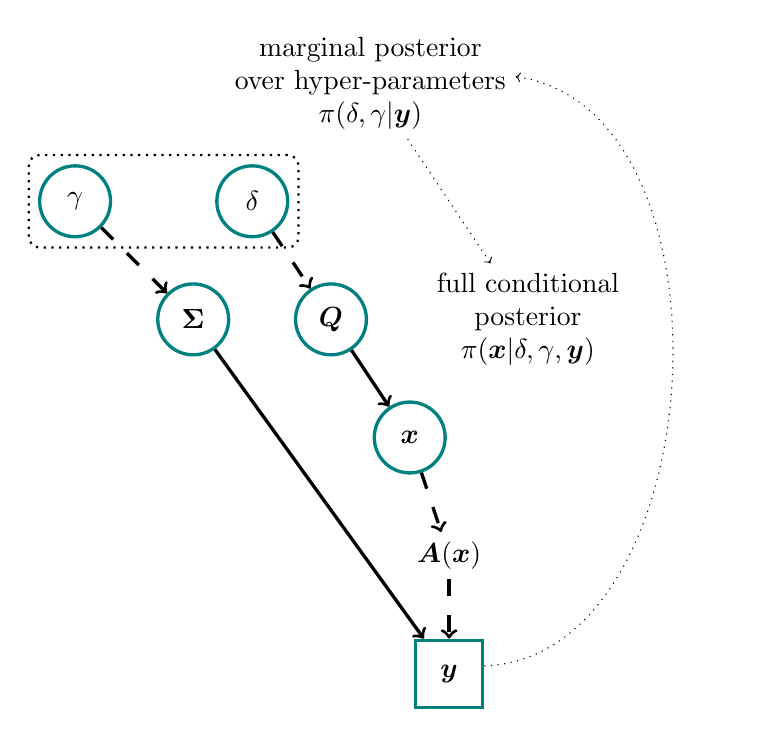
\begin{tikzpicture}
		%box/.style = {draw, thick, minimum width=2.5cm, minimum height=1cm},
		every edge/.style = {draw, -latex, thick} % <---
		\node[roundnode2] at (-2.5,5) (Q)     {$\bm{Q}$};
		\node[roundnode2] at (-1.5,3.5) (x)     {$\bm{x}$};
		\node[align=center] at (-1,2) (A)    {$\bm{A}( \bm{x})$};
		\node[rectnode] at (-1,0.5) (y)    {$\bm{y}$};
		%\node[roundnode2] at (-2.5,2.5) (e)    {$\bm{\eta}$};
		\node[roundnode2] at (-4.25,5) (S)    {$\bm{\Sigma}$};
		\node[roundnode2] at (-5.75,6.5) (s)    {$\gamma$};
		\node[roundnode2] at (-3.5,6.5) (d)    {$\delta$};
		
%		\node[roundnode2] at (-8,10) (shyp)    {$\bm{\theta}_{\gamma}$};
%		\node[roundnode2] at (-5.5,10) (dhyp)    {$\bm{\theta}_{\delta}$};
		%Lines
		\draw[->, very thick] (S) -- (y);
		\draw[->, mydotted, very thick] (s) -- (S);
		%\draw[->, mydotted, very thick] (e) -- (y);
		\draw[->,mydotted,  very thick] (A) -- (y);
		\draw[->, mydotted,  very thick] (x) -- (A);
%		\draw[->, very thick] (shyp) -- (s);
%		\draw[->, very thick] (dhyp) -- (d);
		
		
		\draw[->, mydotted, very thick] (d) -- (Q); 
		
		\draw[->, very thick] (Q) -- (x); 
		%\node[align=center] at (0,4) (f3) {$= \bm{A}$};
		%\node[align=center] at (0.25,3.95) (f3) {$\approx \bm{M A}_L$};
		\node[align =center] at (-2,8) (T1) {marginal posterior \\ over hyper-parameters \\ $\pi(\delta,\gamma  | \bm{y})$};
		\node[align =center] at (0,5) (T2) {full conditional \\ posterior \\ $\pi( \bm{x} | \delta,\gamma, \bm{y})$ };
		
		%\node[align =center] at (-2.5,10) (T3) {hyper-prior distributions \\ $\pi( \delta, \gamma)$ };
		
		\node[fit=(s)(d),draw,thick,dotted,black, rounded corners] {};
		\draw[->,dotted] (y) edge[bend right=85] (T1);  
		\draw[->,dotted] (T1) -- (T2); 
		
	\end{tikzpicture} 
	\caption[Directed acyclic graph for ozone retrieval and MTC scheme.]{DAG for visualisation of the hierarchical modelling process and the conditional dependency between the parameter and the hyper-parameters. The hyper-parameter $\gamma$ deterministically (dotted line) sets the noise covariance $\bm{\Sigma} = \gamma^{-1}\bm{I}$, which then describes the random (solid line) noise vector $\bm{\eta} \sim \mathcal{N}(0,\bm{\Sigma})$.
		The hyper-parameter $\delta$ determines (dotted line) the prior precision matrix $\bm{Q} = \delta \bm{L}$ for the normally distributed (solid line) prior $\bm{x}| \delta \sim \mathcal{N}(0, \bm{Q}^{-1})$, where $\bm{L}$ is a graph Laplacian, see Eq.~\ref{eq:GLapl}.
		The hyper-prior distributions (solid line) $\pi(\delta, \gamma)$ are defined by $\bm{\theta}_{\gamma}$ and $\bm{\theta}_{\delta}$.
		Through the forward model we generate noise-free data $\bm{A}(\bm{x})$ and the obeserved data set $\bm{y}$ includes some added noise $\bm{\eta}$.
		Within the MTC scheme, we evaluate the marginal posterior over the hyper-parameters $\pi(\gamma, \delta | \bm{y})$ first and then the full conditional posterior $\pi(\bm{x}|\delta,\gamma,\bm{y})$. This breaks the correlation structure of $\delta$ and $\gamma$, and $\bm{x}$, and allows us to evaluate the marginal posterior independently of $\bm{x}$.}
	\label{fig:DAGO3}
\end{figure}

The distributions that define the hierarchical Bayesian model are:
\begin{subequations}
	\begin{align}
		\bm{y} |  \bm{x},\delta, \gamma  &\sim \mathcal{N}(\bm{A} \, \bm{x}, \gamma^{-1} \bm{I}) \label{eq:likelihoodAppl} \\
		\bm{x}| \delta  &\sim \mathcal{N}(\bm{0}, (\delta \bm{L})^{-1} ) \label{eq:priorXAppl} \\
		\delta  &\sim \mathcal{T}(\alpha_{\delta}, \beta_{\delta})\label{eq:priorDelAppl} \\
		\gamma  &\sim \mathcal{T}(\alpha_{\gamma}, \beta_{\gamma})\label{eq:priorGamAppl} \, .
	\end{align} 
\end{subequations}
Assuming Gaussian noise $\bm{\eta} \sim \mathcal{N}(0, \gamma^{-1} \bm{I})$, the likelihood function is a normal distribution with mean $\bm{A} \bm{x}$ and covariance matrix $\gamma^{-1} \bm{I}$.
We define a normal prior-distribution $\pi(\bm{x}|\delta)$ with zero mean and precision matrix $\delta \bm{L}$, where $\delta$ is a smoothness hyper-parameter and $\bm{L}$ is a discrete approximation to the second derivate operator (see Eq.~\ref{eq:GLapl}).
Here the hyper-prior distributions $\pi(\delta)$ and $\pi(\gamma)$ are Gamma distributions with shape $\alpha$ and rate $\beta$.

We can visualise this hierarchical structure and the conditional dependencies between hyper-parameters and parameters through a DAG, as in Fig.~\ref{fig:DAGO3}.
The hyper-parameter $\gamma$ sets the noise covariance deterministically (dotted line), but is itself statistically (solid line) defined by the hyper-prior distribution $\pi(\gamma)$.
This is a Gamma distribution, where $\bm{\theta}_{\gamma}$ determines the shape and rate of $\pi(\gamma)$.
Similarly $\bm{\theta}_{\delta}$ defines the Gamma distribution $\pi(\delta)$.
%The prior distribution $\pi(\bm{x}|\delta)$ is a normal distribution with zero mean and precision matrix $\bm{Q}(\delta) =\delta \bm{L}$.
Through the linear forward model the space $\Omega$ is determined by all measurable noise-free data sets $\bm{A}\bm{x}$.
From that space we observe (square box) a data set $\bm{y}$ including some additive noise $\bm{\eta}$.

Given that data, we ``reverse the arrows'' to determine the posterior distribution $\pi(\bm{x}, \delta, \gamma |\bm{y})$ over the parameter $\bm{x}$ and the hyper-parameters $\delta$ and $\gamma$.
%Since noise is a random process with a defined distribution, the posterior distribution $\pi(\bm{x}|\bm{y})$ is well defined.
Usually, due to underlying correlation structures between the parameter and the hyper-parameters, evaluating this posterior poses a significant challenge.
The MTC scheme breaks this correlation and provides the marginal posterior $\pi(\delta, \gamma | \bm{y})$ first and then the full conditional posterior $\pi(\bm{x}|\delta, \gamma,\bm{y})$.
%Since the forward model described in Ch. \ref{ch:formodel} is weakly non-linear we will set up a linear Bayesian hierarchical framework first based on the linear forward model $\bm{A}_L$ and then later the approximated version $\bm{A}_{NL}\bm{M} \bm{A}_L$.
%Furthermore, the noise is normally distributed, so we establish a linear-Gaussian Bayesian hierarchical framework, aiming to recover an ozone profile and a pressure over temperature profile.
%In doing so, we first draw a directed acyclic graph (DAG) to visualise the measurement and modelling process and determine hyper-parameters and correlations between parameters.
%Then we define prior distributions over all parameters as well as a likelihood function so that we can formulate the posterior distribution.

%In this section, we choose the prior distributions and describe the approach to evaluate the posterior distribution for ozone $\pi(\delta, \gamma, \bm{x}|\bm{y})$, including the noise hyper-parameter $\gamma$.
% we define a linear-Gaussian Bayesian hierarchical model, see Sec. \ref{subsec:LinBay},
%\begin{subequations}
%	\begin{align}
	%		\bm{y} |  \bm{x}, \gamma &\sim \mathcal{N}(\bm{A} \bm{x}, \gamma^{-1} \bm{I}) \label{eq:likelihood} \\
	%		\bm{x} |  \delta &\sim \mathcal{N}(\bm{0}, (\delta \bm{L})^{-1}) \label{eq:xPrior} \\
	%		\delta, \gamma &\sim \pi(\delta, \gamma) \label{eq:gammaPrior},
	%	\end{align}
%	\label{eq:O3BayMode}
%\end{subequations}
%with a normally distributed likelihood $\pi(\bm{y} |  \bm{x}, \gamma)$ including the forward model matrix $\bm{A}$ and prior distributions $\pi(\bm{x} |  \delta)$ and $\pi(\delta, \gamma)$, the noise covariance matrix $\gamma^{-1} \bm{I}$, the prior precision matrix $\delta \bm{L}$ and the prior mean set to zero, as in ~\cite{fox2016fast}.
%The chosen Bayesian model is very similar to the regularisation approach, since we like to show that we receive much more meaningful results compared to a single regularisation solution.

\subsubsection{Prior Modelling}
\label{subsec:PriorModelO3}
Completing this Bayesian framework one has to define prior distributions over the hyper-parameters and parameters.
Ideally, we define the prior distributions as uninformative as possible, and include functional dependencies and physical properties.

By choosing a normally distributed prior $\pi(\bm{x}|\delta)$ with zero mean and no other restrictions, it is clear that our model does not take into account that ozone values cannot be negative.
The precision matrix of that prior distribution is
\begin{align}
	\delta \bm{L} =
	\delta
	\begin{bmatrix}
		2 & -1 & & &  \\
		-1 & 2 & -1 & &   \\
		& \ddots & \ddots & \ddots &\\ 
		& & -1 & 2 & -1  \\
		& & & -1 & 2 
	\end{bmatrix} 
	\label{eq:GLapl} 
\end{align}
which is a discrete approximation to the second derivative operator with Dirichlet boundary condition and defines a 1-dimensional Graph Laplacian as in~\cite{wang2015graphs, fox2016fast}.
We reduce the dimension of $\bm{x}$ from $45$ to $n = 34$ by discarding every second ozone VMR over a height of $\approx47$km.
Doing that, while not changing $\bm{L}$ effectively induces a larger correlation between points at higher altitude.

For $\delta$ and $\gamma$ we pick relatively uninformative Gamma distributions so that \linebreak$\gamma \sim \mathcal{T}(\bm{\theta_{\gamma}}) \propto \gamma^{\alpha_\gamma -1 } \exp{( -\beta_\gamma \gamma) } $ and $\delta \sim \mathcal{T}(\bm{\theta_{\delta}})$ with $\bm{\theta_{\gamma}} = \{  \alpha_\gamma, \beta_\gamma\}  = \{ \alpha_\delta ,\beta_\delta\} = \bm{\theta_{\delta}} = (1,10^{-35})$ similar to \cite{fox2016fast}.
Because of those Gamma distributions, $\pi(\gamma | \lambda, \bm{y}) \sim \mathcal{T}(\cdot)$ is a Gamma distribution with $\lambda = \delta / \gamma $ and easy to sample from.


\subsection{Posterior Distribution}
\label{sec:FirstO3Post}
As explained in Sec.~\ref{subsec:TheoMTC}, we factorise the posterior
\begin{align}
	\pi( \bm{x}, \delta, \gamma| \bm{y}) \propto \pi(\bm{y}| \bm{x},\delta,\gamma) \pi( \bm{x},  \delta,\gamma)
\end{align}
into 
\begin{align}
	\pi( \bm{x},  \delta,\gamma| \bm{y}) =\pi( \bm{x}| \delta,\gamma, \bm{y})\pi( \delta,\gamma | \bm{y})
\end{align}
the marginal posterior $\pi(\delta ,\gamma| \bm{y})$ and full conditional posterior $\pi( \bm{x}| \delta,\gamma, \bm{y})$ (see Eq.~\ref{eq:MTC}).
%Fox and Norton call this method the marginal and then conditional method (MTC) \cite{fox2016fast}, where we break the correlation structure between $\bm{x}$ and $\gamma, \delta$ as illustrated in Fig. \ref{fig:RueHeld} by marginalising over $\bm{x}$.
As discussed in~\cite{fox2016fast}, for the linear-Gaussian case, $\bm{x}$ cancels in the marginal posterior over the hyper-parameters.
Following the MTC scheme, we characterise the marginal posterior first and then the full conditional posterior.

\subsubsection{Marginal Posterior}
\label{subsec:FirstMargPost}
For the hierarchical model specified in Eq.~\ref{eq:likelihoodAppl} to Eq.~\ref{eq:priorGamAppl}, the marginal posterior distribution over the hyper-parameters is given by
\begin{align}
	\pi( \lambda,\gamma  | \bm{y}) \propto &  \lambda^{n/2 + \alpha_{\delta}-1} \gamma^{m/2 + \alpha_{\delta} + \alpha_{\gamma}-1}   \exp{ \Bigl\{ - \frac{1}{2} g ( \lambda) - \frac{\gamma}{2} f ( \lambda) - \beta_{\delta} \lambda  \gamma - \beta_{\gamma} \gamma \Bigr\}},
	\label{eq:MargPostTheo}
\end{align}
with the regularisation parameter $\lambda = \delta / \gamma$, and
\begin{subequations}
	\begin{align}
		&f ( \lambda) = \bm{y}^T \bm{y} - (\bm{A}^T \bm{y})^T (\bm{A}^T  \bm{A} + \lambda \bm{L})^{-1} \bm{A}^T \bm{y}  \label{eq:fAppl} \, ,  \\
		&\text{and } g(\lambda) = \log \det (\bm{A}^T  \bm{A} + \lambda \bm{L}) \label{eq:gAppl} \, .
	\end{align}
\end{subequations}
Note that when changing variables from $\delta = \lambda \gamma$ to $\lambda$ the hyper-prior distribution changes to $\pi(\lambda | \gamma) \propto \lambda^{\alpha_{\delta}-1} \gamma^{\alpha_{\delta}} \exp{(- \beta_{\delta} \lambda  \gamma)} $, due to $\text{d}\delta / \text{d} \lambda = \gamma$.
Here, $\lambda$ is introduces as the regularisation parameter \cite{fox2016fast}.
Because of the chosen Gamma priors the conditional marginal posterior 
\begin{align}
	\gamma |  \lambda, \bm{y} &\sim \mathcal{T}\bigg( \frac{m}{2} + \alpha_\delta + \alpha_\gamma, \frac{1}{2} f (\lambda) + \beta_\gamma + \beta_\delta \lambda \bigg)\label{eq:GibbsStep}
\end{align} 
is a Gamma distribution.

\subsubsection{Full Conditional Posterior}
\label{subsec:firstCond}
As in \cite{SIMPSON201216}, consider the joint Gaussian distribution
\begin{align}
	\begin{pmatrix}
		\bm{x} \\
		\bm{y}
	\end{pmatrix}\sim \mathcal{N}\left[  \begin{pmatrix}
		\bm{\mu} \\
		\bm{A}\bm{\mu}
	\end{pmatrix},\begin{pmatrix}
		\bm{Q} + \bm{A}^T \bm{\Sigma}^{-1} \bm{A} & - \bm{A}^T \bm{\Sigma}^{-1} \\
		\bm{\Sigma}^{-1} \bm{A} & \bm{\Sigma}^{-1} 
	\end{pmatrix}^{-1} \right] \, 	\label{eq:jointMultiGaus}
\end{align}
with $\bm{\Sigma}^{-1} = \gamma \bm{I} $ and $\bm{Q}  = \delta \bm{L} $ and $\bm{\mu} = \bm{0}$.
Then the full conditional posterior distribution of ozone 
\begin{align}
	\bm{x}| \delta, \gamma, \bm{y}  \sim \mathcal{N}\big( \underbrace{ (\bm{A}^T \bm{A} + \delta / \gamma \bm{L} )^{-1} \bm{A}^T \bm{y}}_{\bm{x}_{\lambda}}, ( \underbrace{ \gamma \bm{A}^T \bm{A} + \delta \bm{L} }_{\gamma \bm{B}_{\lambda}}  )^{-1} \big) \, \label{eq:CondPost},
\end{align}
is a normal distribution with $\lambda = \delta / \gamma $ and samples can be drawn via the randomise then optimise (RTO) method (see Sec.~\ref{subsec:FullCondPost}).

Alternatively, the posterior mean
\begin{align}
	\bm{\mu}_{\bm{x}|\bm{y}} = \int \bm{x}_{\lambda} \pi(\lambda| \bm{y}) \diff\lambda \approx \sum \bm{x}_{\lambda_i} \pi(\lambda_i| \bm{y}) \, , \label{eq:MeanInt}
\end{align} and posterior covariance
\begin{align}
	\bm{\Sigma}_{\bm{x}|\bm{y}} = \int \gamma^{-1}  \pi(\gamma | \bm{y} ) \, \diff \gamma \, \int  \bm{B}_{\lambda}^{-1} \, \pi(\lambda | \bm{y} )  \, \text{d} \lambda  \approx \sum {\gamma_i}^{-1}\pi(\gamma_i| \bm{y}) \sum \bm{B}_{\lambda_i}^{-1}\pi(\lambda_i| \bm{y})\, \label{eq:CovInt}
\end{align}
of $\pi(\bm{x}| \bm{y})$ can be computed as weighted expectations over the marginal posterior $\pi(\lambda,\gamma | \bm{y})$ by quadrature~\cite[Sec. 2.1]{Dick_Kuo_Sloan_2013} with $\sum \pi(\lambda_i| \bm{y}) = \sum \pi(\gamma_i| \bm{y}) = 1$.
%We use the Cholesky decomposition of $\bm{B}_{\lambda} = \bm{A}^T \bm{A} + \lambda \bm{L}$ to invert $\bm{B}_{\lambda}$ and to calculate $\bm{x}_{\lambda} = (\bm{A}^T \bm{A} + \lambda \bm{L} )^{-1} \bm{A}^T \bm{y}$ both via \texttt{scipy.linalg.cho\_solve}.


\section{Results}
Given the simulated data the problem is treated as a linear inverse problem, neglecting the absorption in the RTE.
The marginal posterior is evaluated on a predefined grid, where the posterior mean is obtained at no additional computational cost.
Samples from the conditional posterior are obtained via the RTO method.
An affine map approximates the non-linear forward model from the linear forward model.
Again, with the approximated forward model, the marginal posterior is calculated on the same predefined grid.
Lastly, the mean and the sample-based STD of the posterior ozone profile are provided.
Recall that $\bm{x} \in \mathbb{R}^n$ with $n = 34$ and $\bm{y} \in \mathbb{R}^m$ with $m = 30$.

\begin{figure}[ht!]
	\centering
    \includegraphics[]{AffinePapData.png}
	\caption[]{Non-linear noise-free data and non-linear noisy data at different tangent heights.}
	\label{fig:Data}
\end{figure} 
\clearpage

\subsection{Marginal Posterior}
\label{sec:firstMarg}
A $N_{\text{grid}}  \times N_{\text{grid}} $ grid for $\lambda = [10^{-5},8 \times 10^{-4}] $ and $\gamma = [0.8\times 10^{15},1.2\times 10^{16}] $ with $N_{\text{grid}} = 25$ grid points is established.
The marginal posterior
\begin{align}
	\pi( \lambda,\gamma  | \bm{y}) \propto &  \lambda^{34/2 } \gamma^{30/2 +1}   \exp{ \Bigl\{ - \frac{1}{2} g ( \lambda) - \frac{\gamma}{2} f ( \lambda) - 10^{-35}\gamma ( \lambda  - 1 )\Bigr\}},
	\label{eq:MargPostAppl}
\end{align}
is evaluated on that grid.
For each evaluation of the marginal posterior, most of the computational effort lies in $f(\lambda)$ and $g(\lambda)$.
For each $\lambda$ on the grid we do a Cholesky decomposition of $\bm{B}_{\lambda} = \bm{A}^T \bm{A} + \delta / \gamma \bm{L}  = \bm{C}^T\bm{C}$ via the Python function \texttt{numpy.linalg.cholesky}.
This immediately gives us  $g(\lambda) = 2 \sum \log \text{diag}(\bm{C})$.
We calculate $\bm{x}_{\lambda} = (\bm{A}^T \bm{A} + \lambda \bm{L} )^{-1} \bm{A}^T \bm{y}$ via \texttt{scipy.linalg.cho\_solve} which then gives us $f(\lambda) = \bm{y}^T \bm{y} - (\bm{A}^T \bm{y})^T \bm{x}_{\lambda}$.
Then for each $\lambda$ the cost to compute the marginal posterior $\pi( \lambda,\cdot | \bm{y})$ for varying $\gamma = [0.8\times 10^{15},1.2\times 10^{16}] $ is negligible.
\begin{figure}[ht!]
	\centering
	\includegraphics[]{AffinePapFirstMarg.png}
	\caption[]{Marginal posterior for linear forward model on a $20 \times 20$ grid.}
	\label{fig:FirstMar}
\end{figure}


Further, the posterior mean in Eq.~\ref{eq:MeanInt} is obtained by weighted expatiation over the predefined grid with $\pi(\lambda| \bm{y}) = \int \pi(\lambda, \gamma| \bm{y}) \diff \gamma $ at no additional computational cost.
We normalise numerically over the grid so that $\sum \pi(\lambda_i| \bm{y}) = 1$.

\subsubsection{Sampling from Marginal posterior}
Independent samples $\lambda^{(k)},\gamma^{(k)}  \sim \pi_{\lambda,\gamma }( \cdot | \bm{y}) $ from the Marginal posterior are needed if one wants to draw an ozone sample from the full conditional posterior $\bm{x}^{(k)}  \sim \pi_{\bm{x}}( \cdot|\lambda^{(k)},\gamma^{(k)}  , \bm{y})$.

We sample from the marginal posterior via the inverse Rosenblatt transport (IRT) scheme as in~\cite{dolgov2020approximation}.
A seed $\bm{u}^{(k)} \sim \mathcal{U}(0,1)^d$, where $d=2$ and $\bm{u}^{(k)} = \{u^{(k)}_1,u^{(k)}_2 \}$, from the uniform distribution is projected onto the hyper-parameter space via the cumulative distribution function (CDF) 
\begin{align}
	F(\lambda) = \int_{- \infty}^\lambda \pi(\lambda^{\prime}| \bm{y}) \diff \lambda^{\prime} \, ,
\end{align}
where $\pi(\lambda| \bm{y})  = \sum_{\gamma} \pi(\lambda, \gamma| \bm{y}) $ on the predefined grid.
The inverse
\begin{align}
	\lambda^{(k)} |\bm{y} = F^{-1}(u^{(k)}_1) \, 
\end{align}
provides a sample from $\pi(\lambda| \bm{y}) $.
In order to draw an samples $\gamma^{(k)} |  \lambda^{(k)}, \bm{y}$ we repeat this procedure.
$\pi(\gamma |  \lambda^{(k)}, \bm{y})$ (see Eq.~\ref{eq:MargPostAppl}) is calculated for the every $\gamma$ value on the grid with fixed $\lambda^{(k)}$.
Here we use piecewise linear interpolation via the Python function \texttt{numpy.linalg.interp} to obtain the values $f( \lambda^{(k)})$ and $g( \lambda^{(k)})$ (see Fig.~\ref{fig:fandg}).
Then the CDF
\begin{align}
	F(\gamma) = \int_{- \infty}^\gamma \pi(\gamma |  \lambda^{(k)}, \bm{y}) \diff \gamma^{\prime} \, 
\end{align}
is calculated and an independent sample is given as:
\begin{align}
	\gamma^{(k)}|\lambda^{(k)} , \bm{y} = F^{-1}(u^{(k)}_2) \, .
\end{align}
Note that alternatively one could draw an independent sample using Eq.~\ref{eq:GibbsStep}, which is a Gamma distribution due to the choice of prior.
The presented IRT works for arbitrary priors.
\begin{figure}[ht!]
	\centering
	\includegraphics[]{AffinePapfandg.png}
	\caption[]{Functions $f(\lambda)$ and $g(\lambda)$ for $\lambda = [10^{-5},8 \times 10^{-4}] $, grid points are marked red. True function values between grid points are plotted in black.}
	\label{fig:fandg}
\end{figure} 

In theory, this scheme provides independent samples, but in practice, every system produces correlated samples.
To assess how efficient this scheme is, we define the Integrated Autocorrelation Times (IACT)
\begin{align}
	\tau_{\text{int}}  \coloneqq  \Bigg(  1 + 2 \sum_{t = 1}^{W} \frac{\Gamma(t)}{\Gamma(0)}  \Bigg)  
\end{align} 
as in \cite{fox2016fast} with an autocorrelation coefficient $\Gamma(t)$.
This is twice the value of the IACT in~\cite[pp. 103-105]{wolff2002LecNot} and~\cite{wolff2004monte,drikHesse}, as commonly defined within the physics community.
U. Wolff~\cite{wolff2004monte} (and the Python implementation by D. Hesse~\cite{drikHesse}) provide a way to not only calculate the IACT safely but also to quantify the errors of the estimated IACT.
The IATCs are $\tau_{\text{int},\lambda} = 1.05\pm0.04$ and $\tau_{\text{int},\gamma} =0.99\pm0.03$ based on a chain with 10000 samples.
So every second sample via the IRT scheme presents an independent marginal posterior sample.
Conditioned on an independent sample from the marginal posterior, one can draw an independent sample from the full conditional posterior.


\subsection{Full Conditional Posterior}
\label{subsec:FullCondPost}
To sample an posterior ozone profile from the full conditional $\pi(\bm{x} | \delta, \gamma, \bm{y})$ with $\delta = \lambda \gamma$ we use the RTO method, as in~\cite{bardsley2012mcmc, bardsley2014randomize,BardsleyTC2019RTO,fox2016fast}.
Rewrite the full conditional posterior as
\begin{align}
	\pi(\bm{x} |  \delta, \gamma, \bm{y}) & \propto \pi(\bm{y}|\bm{x}, \gamma) \pi(\bm{x}| \delta)\\
	&\propto \exp \left(-\frac{1}{2} (\bm{A} \bm{x} - \bm{y})^T \bm{\Sigma}^{-1} (\bm{A}  \bm{x} - \bm{y})\right) \exp \left(-\frac{1}{2} (\bm{\mu} - \bm{x} )^T \bm{Q}(\bm{\mu} - \bm{x} ) \right),\\
	& = \exp \left( - \frac{1}{2}\left\lVert \hat{\bm{A}} \bm{x} - \hat{\bm{y}} \right\rVert_{L^2}^2 \right),
\end{align}
where
\begin{align}
	\label{eq:minimizer}
	\hat{\bm{A}} \coloneqq 
	\begin{bmatrix}
		\bm{\Sigma}^{-1/2} \bm{A} \ \\
		\bm{Q}^{1/2}
	\end{bmatrix}, \quad 
	\hat{\bm{y}} \coloneqq 
	\begin{bmatrix}
		\bm{\Sigma}^{-1/2} \bm{y} \\
		\bm{Q}^{1/2} \bm{\mu}
	\end{bmatrix} , 
\end{align}
$\bm{Q} = \delta \bm{L}$ is the prior precision, $\bm{\mu} = \bm{0}$ the prior mean and $\bm{\Sigma}= \gamma^{-1} \bm{I}$ the noise covariance.
A sample $\bm{x}^{(k)}$ from the full conditional posterior $ \pi(\bm{x}|   \delta, \gamma,  \bm{y})$ is obtained by minimising the following equation:
\begin{align}
	\bm{x}^{(k)} = \arg \min_{\bm{x}} \lVert \hat{\bm{A}} \bm{x} - ( \hat{\bm{y}} + \bm{b} ) \rVert_{L^2}^2 
\end{align}
with a random additive perturbation $\bm{b} \sim \mathcal{N}(\bm{0}, \bm{I})$.
This expression becomes
\begin{align}
	\label{eq:RTO}
	\left( \bm{A}^T \bm{\Sigma}^{-1} \bm{A} + \bm{Q} \right) \bm{x}^{(k)} = \bm{A}^T \bm{\Sigma}^{-1} \bm{y} + \bm{Q} \bm{\mu} + \bm{v}_1 + \bm{v}_2,
\end{align}
%where the term $-\hat{\bm{A}}^T \bm{b}$ is decomposed as $\bm{v}_1 + \bm{v}_2$, 
with $\bm{v}_1 \sim \mathcal{N}(\bm{0}, \bm{A}^T \bm{\Sigma}^{-1} \bm{A})$ and $\bm{v}_2 \sim \mathcal{N}(\bm{0}, \bm{Q}^{-1})$, representing independent Gaussian random variables~\cite{bardsley2012mcmc, fox2016fast}.

More explicitly, conditioned on an independent $\lambda^{(k)},\gamma^{(k)} \sim \pi_{\lambda,\gamma }(\cdot | \bm{y})$, one independent full conditional posterior sample is given as  
\begin{align}
	\label{eq:RTOAppl}
	\bm{x}^{(k)} = 	\Big(  \underbrace{\gamma^{(k)} \bm{A}^T\bm{A} +  \delta^{(k)}\bm{L}}_{\bm{B}^{(k)}} \Big)^{-1} \left(  \gamma^{(k)}  \bm{A}^T\bm{y} +\sqrt{\gamma^{(k)}} \bm{A}^T \tilde{\bm{v}}_1 + \sqrt{\delta^{(k)}}\bm{L}^{1/2}\tilde{\bm{v}}_2\right)
\end{align}
with $\tilde{\bm{v}}_1 \sim \mathcal{N}(\bm{0},  \bm{I})$, $\tilde{\bm{v}}_2 \sim \mathcal{N}(\bm{0}, \bm{I} )$ and $\bm{L}^{1/2}$ is the Cholesky decomposition of $\bm{L}$ \cite{bardsley2012mcmc}.
Note that $\bm{v}_1 \in \mathbb{R}^m$ and $\bm{v}_2 \in \mathbb{R}^n$.
The Cholesky factorisation of $\bm{B}^{(k)}$ and $\bm{L}$ is obtained via the Python function \texttt{numpy.linalg.cholesky} and \texttt{scipy.linalg.cho\_solve} is used to solve for $\bm{x}^{(k)}$.
We draw $n-1 = 29$ posterior samples in $\approx 0.003$.
The full conditional posterior samples are plotted in Fig.~\ref{fig:OzonSampl} with negative ozone values set to zero.
The fact that we have to deal with negative ozone values is due to the poor prior choice in $\pi(\bm{x}|\delta)$.
Those full conditional ozone samples are used to find an affine map.


\begin{figure}[ht!]
	\centering
    \includegraphics[]{AffinePapOzonSampl.png}
	\caption[]{29 Ozone samples via RTO method and posterior ozone mean via quadrature (see Eq.~\ref{eq:MeanInt}).}
	\label{fig:OzonSampl}
\end{figure}
\clearpage

\subsection{Affine Approximation of the Non-Linear Model}
\label{ch:affine}

\newcommand*{\vertbar}{\rule[-1ex]{0.5pt}{2.5ex}}
\newcommand*{\horzbar}{\rule[.5ex]{2.5ex}{0.5pt}}
The forward map poses a weakly non-linear forward problem.
One could tackle this non-linear inverse problem by fixing the absorption at a previously obtained parameter state and treating this as a linear inverse problem.
After each parameter sample the absorption is then iteratively updated.
Instead, as in Fig.~\ref{fig:affinStrat} illustrated, we approximate the non-linear model using an affine map, which is a linear map with a translation, e.g., $\bm{A}\bm{x} + \bm{b}$.
An affine map $ \bm{z} = \bm{A}\bm{x} + \bm{b}$ maps a Gaussian $\bm{x} \sim \mathcal{N}(\bm{\mu}, \bm{\Sigma})$ onto a Gaussian $\bm{z} \sim \mathcal{N}(\bm{A}\bm{\mu} + \bm{b}, \bm{A}^T\bm{\Sigma}\bm{A})$.

Here we find an affine map $\bm{M}$ that provides a mapping from the linear forward model $\bm{A}_L$ to the non-linear model $\bm{A}(\bm{x})$ for parameters $\bm{x}$ near the posterior mean $\bm{\mu}_{\bm{x}|\bm{y}}$.
%\begin{figure}[htb!]
%	\centering
%	\begin{tikzpicture}
%		\node[rectnode] at (0,0) (Oy)    {$\bm{y}$};
%		\node[roundnode2] at (0,-2) (x)     {$\bm{x}$};
%		\node[roundnode2] at (1.75,-4) (V)    {$\bm{V}$};%{$\bm{A}_{NL}\bm{x}$};
%		\node[roundnode2] at (-1.75,-4) (W)    {$\bm{W}$};%{$\bm{A}_L\bm{x}$};
%		\draw[->, very thick] (Oy.south) -- (x.north); 
%		\draw[->, very thick] (x) -- (V); 
%		\draw[->, very thick] (x) -- (W); 
%		\draw[->, very thick] (W.east) --  (V.west); 
%		\node[align=center] at (1,0) (l1) {data};
%		\node[align=center] at (3.5,-2) (f2) {ozone profiles from $\pi(\bm{x}|\bm{y}) $};
%		\node[align=center] at (1.75,-1) (l1) {$\pi(\lambda , \gamma  | \bm{y})$ with $\bm{A}_L$};
%		
%		
%		\node[align=center] at (-4.25,-4) (f3) {linear forward model};
%		\node[align=center] at (4.75,-4) (f4) {non-linear forward model};
%		\node[align=center] at (0,-5) (f5) {$\bm{A}(\bm{x}) \approx \bm{M A}_L \bm{x}$ };
%		
%		\node[align=center] at (0,-4) (f5) {affine map \\ $\bm{M}$};
%		
%	\end{tikzpicture}
%	\caption[Strategy to find affine map.]{The strategy to find the affine map consists of evaluating the marginal posterior for ozone $\pi(\lambda , \gamma  | \bm{y})$ for the linear forward model. For some ozone samples from the posterior the noise-free linear data $\bm{A}_L \bm{x}$ is calculated to form $\bm{W}$ and similarly $\bm{V}$ is composed using the non-linear model $\bm{A}(\bm{x})$. An affine map $\bm{M}$ approximates the non-linear model from the linear model.}
%	\label{fig:affinStrat}
%\end{figure}

\begin{figure}[htb!]
	\centering
	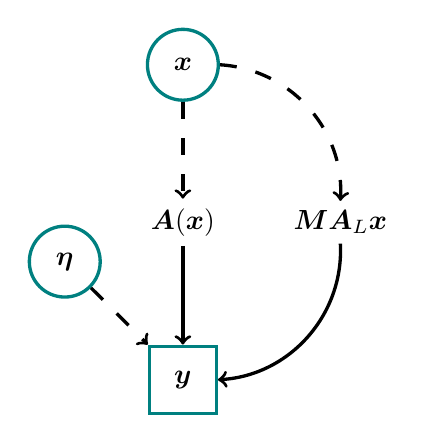
\begin{tikzpicture}
				\node[roundnode2] at (-1,5) (x)     {$\bm{x}$};
		\node[align=center] at (-1,3) (A)    {$\bm{A} (\bm{x})$};
			\node[align=center] at (1,3) (Aff)    {$\bm{M}\bm{A}_L\bm{x}$};
		\node[rectnode] at (-1,1) (y)    {$\bm{y}$};

		\node[roundnode2] at (-2.5,2.5) (e)    {$\bm{\eta}$};
		\draw[->, mydotted, very thick] (e) -- (y);
		\draw[->, very thick] (A) -- (y);
		\draw[->, mydotted,  very thick] (x) -- (A);

		\draw[->,  mydotted, very thick] (x) edge[bend left=45] (Aff);  

		\draw[->, very thick] (Aff) edge[bend left=45] (y);  
		
	\end{tikzpicture}
	\caption[]{Schematic of how the affine map  and the linear forward model approximates the non-linear forward model.}
	\label{fig:affinStrat}
\end{figure}

\subsubsection{Finding an Affine Map}
\label{sec:affine}
We find an affine map by creating the vector spaces $\bm{W}$ based on the linear forward model and $\bm{V}$ based on the non-linear forward model with ground truth pressure and temperature.
More specifically $m-1$ samples $\bm{x}^{(j)} \sim \pi_{\bm{x}}(\cdot|\delta^{(j)} , \gamma^{(j)},\bm{y})$, for $j = 2, \dots,m$, from the posterior and the posterior mean $\bm{\mu}_{\bm{x}|\bm{y}}$ generate,
\begin{align*}
	\bm{W} = \begin{bmatrix}
		\vert& \vert&   &  \vert & & \vert \\
		\bm{A}_{L}  \bm{\mu}_{\bm{x}|\bm{y}} & \bm{A}_{L}  \bm{x}^{(2)}   &  \cdots& \bm{A}_{L} \bm{x}^{(j)} &  \cdots & \bm{A}_{L} \bm{x}^{(m)} \\
		\vert& \vert&   &  \vert & & \vert 
	\end{bmatrix}
	\in \mathbb{R}^{m \times m}
\end{align*}\noindent and
\begin{align*}
	\bm{V} = \begin{bmatrix}
		\vert& \vert&   &  \vert & & \vert \\
		\bm{A}(\bm{\mu}_{\bm{x}|\bm{y}} ) & \bm{A}(\bm{x}^{(2)}) &  \cdots& \bm{A}(\bm{x}^{(j)}) &  \cdots & \bm{A} (\bm{x}^{(m)})  \\
		\vert&\vert&   &  \vert & & \vert 
	\end{bmatrix} = 
	\begin{bmatrix}
		\begin{array}{ccc}
			\horzbar & v_{1} & \horzbar \\
			& \vdots    &          \\
			\horzbar & v_{j} & \horzbar \\
			& \vdots    &          \\
			\horzbar &v_{m} & \horzbar
		\end{array}
	\end{bmatrix}\in \mathbb{R}^{m \times m} \, .
\end{align*}
Then the non-linear forward model is approximated as 
\begin{align}
	\bm{A}(\bm{x}) \approx \bm{M A}_L \bm{x} \, , \label{eq:AffineM}
\end{align}
where we solve $v_j =r_j \bm{W}$ for each row $r_j$ in
\begin{align*}
	\bm{V}\bm{W}^{-1} = \bm{M} =
	\begin{bmatrix}
		\begin{array}{ccc}
			\horzbar & r_{1} & \horzbar \\
			& \vdots    &          \\
			\horzbar & r_{j} & \horzbar \\
			& \vdots    &          \\
			\horzbar &r_{m} & \horzbar
		\end{array}
	\end{bmatrix}\, \in \mathbb{R}^{m \times m} .
\end{align*}
using the Python function \texttt{numpy.linalg.solve}.
This is feasible since every noise-free measurement is independent of each other, and then every row $v_j$ of $\bm{V} \in \mathbb{R}^{m \times m}$ is independent of each other as well.
For an $\bm{x} = \bm{\mu}_{\bm{x}|\bm{y}} + \Delta \bm{x}$ we rewrite Eq.~\ref{eq:AffineM} to
\begin{align}
	\bm{A}(\bm{x})  \approx \underbrace{  \bm{M A}_L  \bm{\mu}_{\bm{x}|\bm{y}} }_{= \bm{A}( \bm{\mu}_{\bm{x}|\bm{y}} )  }+  \underbrace{\bm{M A}_L  \Delta \bm{x} }_{= \bm{A}^{\prime}( \bm{\mu}_{\bm{x}|\bm{y}} )  \Delta \bm{x} }\,  \label{eq:AffineTaylor}\\
	=    \underbrace{ \bm{A}^{\prime}( \bm{\mu}_{\bm{x}|\bm{y}} ) \bm{x}}_{ \bm{A}\bm{x}}  +  \underbrace{ \bm{A}( \bm{\mu}_{\bm{x}|\bm{y}} )  - \bm{A}^{\prime}( \bm{\mu}_{\bm{x}|\bm{y}} ) \bm{\mu}_{\bm{x}|\bm{y}}}_{  \bm{b}} 
\end{align}
to show that $ \bm{M}:\bm{A}_L\bm{x} \rightarrow \bm{A}(\bm{x})$ is an affine map.

\begin{figure}[ht!]
	\centering
	\includegraphics{AffinePapAssMap.png}
	\caption[Assessment of affine map.]{Assessment of how well the affine map $\bm{M}$ approximates noise-free non-linear data $\bm{A}(\bm{x})$ (red circles) from noise-free linear data $\bm{A}_L\bm{x}$ (grey stars). The approximated noise-free data (black stars) has a relative RMS error of $\approx 0.01\%$ compared to the true non-linear noise-free data.
		The ozone profile $\bm{x}$ to generate this noise-free data has not been used to create the affine map.}
	\label{fig:AssMap}
\end{figure}
The relative RMS difference $\lVert \text{vec}(\bm{M}\bm{W}) - \text{vec}(\bm{V})  \rVert_{L^2} / \lVert \text{vec}(\bm{M}\bm{W}) \rVert_{L^2} $ between the mapped linear noise-free data and the non-linear noise-free data is approximately $0.001\%$.
This is much smaller than the relative RMS difference between $\bm{W}$ and $\bm{V}$ of about $1\%$.
Here $\text{vec}(\bm{V})$ vectorises the matrix $\bm{V}$.
Fig.~\ref{fig:AssMap} shows the mapping for one posterior ozone sample with a relative RMS error~$\approx0.01\%$.
This posterior ozone sample has not been used to create this mapping; in other words, this is an unseen event not occurring in the training data.
Consequently, from here onwards the approximated forward map is used.
This takes $\approx 0.1$s.

\clearpage
\subsection{Posterior ozone}
The linear forward model that approximates the non-linear forward model is defined as
\begin{align}
	\bm{A} \coloneqq \bm{M} \bm{A}_L \, .
\end{align}

We use the exact same grid and setup as in Sec.~\ref{sec:firstMarg} to define the marginal posterior (see Fig.~\ref{fig:MargFinal}).
\begin{figure}[ht!]
	\centering
	\includegraphics[]{AffinePapMargFinal.png}
	\caption[]{Marginal posterior for approximated forward model on a $20 \times 20$ grid.}
	\label{fig:MargFinal}
\end{figure}
As already mentioned, that gives us the posterior mean via weighted expectation for free.
The IATCs of the marginal posterior samples are $\tau_{\text{int},\lambda} = 0.97 \pm0.03$ and $\tau_{\text{int},\gamma} =0.95\pm0.03$ based on a chain with length of 10000.
Hence, every second sample is an independent sample from the marginal posterior.

Samples from the conditional posterior are drawn via the RTO method.
To estimate the number of samples needed for a good enough estimate of the STD, we calculate the average Coefficient of Variation ($\overline{\text{CV}}$),
\begin{align}
	\overline{\text{CV}} = \frac{1}{n}  \left\lVert  \frac{\sqrt{ \text{var}_N(\bm{\mu}_{\bm{x}|\bm{y}})}}{\bm{\mu}_{\bm{x}|\bm{y}} }\right\rVert_1 , \label{eq:avrgCV}
\end{align}
recall that  $\bm{\mu}_{\bm{x}|\bm{y}} \in \mathbb{R}^n$ with $n = 34$.
The $\overline{\text{CV}}$ gives a measure of how much the STD varies compared to the mean.

If the STD is large compared to the mean the $\overline{\text{CV}}$ is large, if the STD is small compared to the mean the $\overline{\text{CV}}$ is small and a rather accurate estimate of the STD is needed.
The sample-based estimate of the variance
\begin{align}
	\text{var}_N(\mu_{\bm{x}|\bm{y}}) =\frac{1}{N-1} \sum^N_{k=1}(\bm{x}^{(k)} - \mu_{\bm{x}|\bm{y}})^T (\bm{x}^{(k)} - \mu_{\bm{x}|\bm{y}})
\end{align}
is calculated with the posterior mean $\mu_{\bm{x}|\bm{y}}$ given by weighted expectations as in Eq.~\ref{eq:MeanInt}.
Alternatively, one could evaluate the posterior covariance as a weighted expectation over the marginal posterior grid (see Eq.~\ref{eq:CovInt}).

The $\overline{\text{CV}}$ is calculated for each number of samples ranging from $1$ to $10^3$ and plotted in Fig.~\ref{fig:Err}.
\begin{figure}[ht!]
	\centering
	\includegraphics[]{AffinePapCV.png}
	\caption[]{Average Coefficient of Variation in $\%$ as calculated in Eq.~\ref{eq:avrgCV}.}
	\label{fig:Err}
\end{figure}
Fig.~\ref{fig:Err} shows that the $\overline{\text{CV}}$ is rather large, indicating that the STD is large compared to the posterior mean.
Further, we conclude that 50 full conditional posterior ozone samples are enough for a sufficient estimate of the STD.
Approximating the marginal posterior on a $20 \times 20$ grid and taking 50 independent full posterior samples of ozone takes $\approx 0.008$s.
The sample-based STD with the posterior mean (via weighted expectation) is plotted in Fig.~\ref{fig:OzoFinal}.
Note that the posterior ozone profile does not capture the second ozone peak at around $80$km.

\begin{figure}[ht!]
	\centering
	\includegraphics[]{AffinePapOzoFinal.png}
	\caption[]{Posterior ozone mean via quadrature (see Eq.~\ref{eq:MeanInt}) and STD based on 20 samples via the RTO method.}
	\label{fig:OzoFinal}
\end{figure}



\clearpage
\section{Conclusion}
\begin{itemize}
    \item $20$ solves of $x_{\lambda}$ for marginal posteirior and full posterior mean (see Eq.~\ref{eq:CondPost} and Eq.~\ref{eq:MeanInt})
	\item $29$ samples of full conditional posterior are enough  for finding an affine map, this includes $29$ solves of ``randomised'' $x_{\lambda}$ via the RTO method (see Eq.~\ref{eq:RTOAppl})
	\item $50$ samples of full conditional posterior are enough for the STD estimate of posterior ozone, this includes $50$ solves of ``randomised'' $x_{\lambda}$ via the RTO method (see Eq.~\ref{eq:RTOAppl})
\end{itemize}
\clearpage
% {\renewcommand*\MakeUppercase[1]{#1}%
% 	\printbibliography[heading=bibintoc,title={\bibtitle}]}
\printbibliography[heading=bibintoc,title={\bibtitle}]

\end{document}
